\documentclass[]{article}
\usepackage{lmodern}
\usepackage{amssymb,amsmath}
\usepackage{ifxetex,ifluatex}
\usepackage{fixltx2e} % provides \textsubscript
\ifnum 0\ifxetex 1\fi\ifluatex 1\fi=0 % if pdftex
  \usepackage[T1]{fontenc}
  \usepackage[utf8]{inputenc}
\else % if luatex or xelatex
  \ifxetex
    \usepackage{mathspec}
  \else
    \usepackage{fontspec}
  \fi
  \defaultfontfeatures{Ligatures=TeX,Scale=MatchLowercase}
\fi
% use upquote if available, for straight quotes in verbatim environments
\IfFileExists{upquote.sty}{\usepackage{upquote}}{}
% use microtype if available
\IfFileExists{microtype.sty}{%
\usepackage{microtype}
\UseMicrotypeSet[protrusion]{basicmath} % disable protrusion for tt fonts
}{}
\usepackage[margin=.75in]{geometry}
\usepackage{hyperref}
\hypersetup{unicode=true,
            pdfborder={0 0 0},
            breaklinks=true}
\urlstyle{same}  % don't use monospace font for urls
\usepackage{color}
\usepackage{fancyvrb}
\newcommand{\VerbBar}{|}
\newcommand{\VERB}{\Verb[commandchars=\\\{\}]}
\DefineVerbatimEnvironment{Highlighting}{Verbatim}{commandchars=\\\{\}}
% Add ',fontsize=\small' for more characters per line
\usepackage{framed}
\definecolor{shadecolor}{RGB}{248,248,248}
\newenvironment{Shaded}{\begin{snugshade}}{\end{snugshade}}
\newcommand{\KeywordTok}[1]{\textcolor[rgb]{0.13,0.29,0.53}{\textbf{#1}}}
\newcommand{\DataTypeTok}[1]{\textcolor[rgb]{0.13,0.29,0.53}{#1}}
\newcommand{\DecValTok}[1]{\textcolor[rgb]{0.00,0.00,0.81}{#1}}
\newcommand{\BaseNTok}[1]{\textcolor[rgb]{0.00,0.00,0.81}{#1}}
\newcommand{\FloatTok}[1]{\textcolor[rgb]{0.00,0.00,0.81}{#1}}
\newcommand{\ConstantTok}[1]{\textcolor[rgb]{0.00,0.00,0.00}{#1}}
\newcommand{\CharTok}[1]{\textcolor[rgb]{0.31,0.60,0.02}{#1}}
\newcommand{\SpecialCharTok}[1]{\textcolor[rgb]{0.00,0.00,0.00}{#1}}
\newcommand{\StringTok}[1]{\textcolor[rgb]{0.31,0.60,0.02}{#1}}
\newcommand{\VerbatimStringTok}[1]{\textcolor[rgb]{0.31,0.60,0.02}{#1}}
\newcommand{\SpecialStringTok}[1]{\textcolor[rgb]{0.31,0.60,0.02}{#1}}
\newcommand{\ImportTok}[1]{#1}
\newcommand{\CommentTok}[1]{\textcolor[rgb]{0.56,0.35,0.01}{\textit{#1}}}
\newcommand{\DocumentationTok}[1]{\textcolor[rgb]{0.56,0.35,0.01}{\textbf{\textit{#1}}}}
\newcommand{\AnnotationTok}[1]{\textcolor[rgb]{0.56,0.35,0.01}{\textbf{\textit{#1}}}}
\newcommand{\CommentVarTok}[1]{\textcolor[rgb]{0.56,0.35,0.01}{\textbf{\textit{#1}}}}
\newcommand{\OtherTok}[1]{\textcolor[rgb]{0.56,0.35,0.01}{#1}}
\newcommand{\FunctionTok}[1]{\textcolor[rgb]{0.00,0.00,0.00}{#1}}
\newcommand{\VariableTok}[1]{\textcolor[rgb]{0.00,0.00,0.00}{#1}}
\newcommand{\ControlFlowTok}[1]{\textcolor[rgb]{0.13,0.29,0.53}{\textbf{#1}}}
\newcommand{\OperatorTok}[1]{\textcolor[rgb]{0.81,0.36,0.00}{\textbf{#1}}}
\newcommand{\BuiltInTok}[1]{#1}
\newcommand{\ExtensionTok}[1]{#1}
\newcommand{\PreprocessorTok}[1]{\textcolor[rgb]{0.56,0.35,0.01}{\textit{#1}}}
\newcommand{\AttributeTok}[1]{\textcolor[rgb]{0.77,0.63,0.00}{#1}}
\newcommand{\RegionMarkerTok}[1]{#1}
\newcommand{\InformationTok}[1]{\textcolor[rgb]{0.56,0.35,0.01}{\textbf{\textit{#1}}}}
\newcommand{\WarningTok}[1]{\textcolor[rgb]{0.56,0.35,0.01}{\textbf{\textit{#1}}}}
\newcommand{\AlertTok}[1]{\textcolor[rgb]{0.94,0.16,0.16}{#1}}
\newcommand{\ErrorTok}[1]{\textcolor[rgb]{0.64,0.00,0.00}{\textbf{#1}}}
\newcommand{\NormalTok}[1]{#1}
\usepackage{graphicx,grffile}
\makeatletter
\def\maxwidth{\ifdim\Gin@nat@width>\linewidth\linewidth\else\Gin@nat@width\fi}
\def\maxheight{\ifdim\Gin@nat@height>\textheight\textheight\else\Gin@nat@height\fi}
\makeatother
% Scale images if necessary, so that they will not overflow the page
% margins by default, and it is still possible to overwrite the defaults
% using explicit options in \includegraphics[width, height, ...]{}
\setkeys{Gin}{width=\maxwidth,height=\maxheight,keepaspectratio}
\IfFileExists{parskip.sty}{%
\usepackage{parskip}
}{% else
\setlength{\parindent}{0pt}
\setlength{\parskip}{6pt plus 2pt minus 1pt}
}
\setlength{\emergencystretch}{3em}  % prevent overfull lines
\providecommand{\tightlist}{%
  \setlength{\itemsep}{0pt}\setlength{\parskip}{0pt}}
\setcounter{secnumdepth}{0}
% Redefines (sub)paragraphs to behave more like sections
\ifx\paragraph\undefined\else
\let\oldparagraph\paragraph
\renewcommand{\paragraph}[1]{\oldparagraph{#1}\mbox{}}
\fi
\ifx\subparagraph\undefined\else
\let\oldsubparagraph\subparagraph
\renewcommand{\subparagraph}[1]{\oldsubparagraph{#1}\mbox{}}
\fi

%%% Use protect on footnotes to avoid problems with footnotes in titles
\let\rmarkdownfootnote\footnote%
\def\footnote{\protect\rmarkdownfootnote}

%%% Change title format to be more compact
\usepackage{titling}

% Create subtitle command for use in maketitle
\newcommand{\subtitle}[1]{
  \posttitle{
    \begin{center}\large#1\end{center}
    }
}

\setlength{\droptitle}{-2em}
  \title{}
  \pretitle{\vspace{\droptitle}}
  \posttitle{}
  \author{}
  \preauthor{}\postauthor{}
  \date{}
  \predate{}\postdate{}


\begin{document}

Michael Leibert

Math 504

Homework 12

~

\begin{itemize} 


\item[2.] In this problem you will implement a neural network to solve a classification problem.   To keep things simple - since time is limited - the data will consist of covariates $x^{(i)} \in \mathbb{R}^2$ and a response $y_i \in \{0,1\}$ for $i=1,2,\dots,N$ (notice $y$ takes on only two possible values).  The classification problem involves fitting the model $y \sim f(x)$ over functions $f(x)$ that can be parameterized by our neural net, which is described below.   The attached file \verb+nn.txt+ contains the samples.  Each sample, corresponding to a row in the file, gives the three values $(x^{(i)}_1, x^{(i)}_2, y_i)$.  
\end{itemize}

~

\begin{itemize} \item[(a)] Visualize the dataset by plotting it with different colors for the two classes of $y$.  
\end{itemize}

~

\begin{Shaded}
\begin{Highlighting}[]
\KeywordTok{setwd}\NormalTok{(}\StringTok{"G:}\CharTok{\textbackslash{}\textbackslash{}}\StringTok{math}\CharTok{\textbackslash{}\textbackslash{}}\StringTok{504"}\NormalTok{);}\KeywordTok{require}\NormalTok{(ggplot2,}\DataTypeTok{quietly=}\NormalTok{T)}
\NormalTok{nn<-}\KeywordTok{read.table}\NormalTok{(}\StringTok{"nn.txt"}\NormalTok{,}\DataTypeTok{header=}\NormalTok{T)   }
\NormalTok{p <-}\StringTok{ }\KeywordTok{ggplot}\NormalTok{(nn, }\KeywordTok{aes}\NormalTok{(x1, x2)) }\OperatorTok{+}\StringTok{ }\KeywordTok{geom_point}\NormalTok{(}\KeywordTok{aes}\NormalTok{(}\DataTypeTok{colour =} \KeywordTok{factor}\NormalTok{(y))) }\OperatorTok{+}\StringTok{   }
\StringTok{  }\KeywordTok{theme}\NormalTok{(}\DataTypeTok{legend.position=}\StringTok{"bottom"}\NormalTok{);p }
\end{Highlighting}
\end{Shaded}

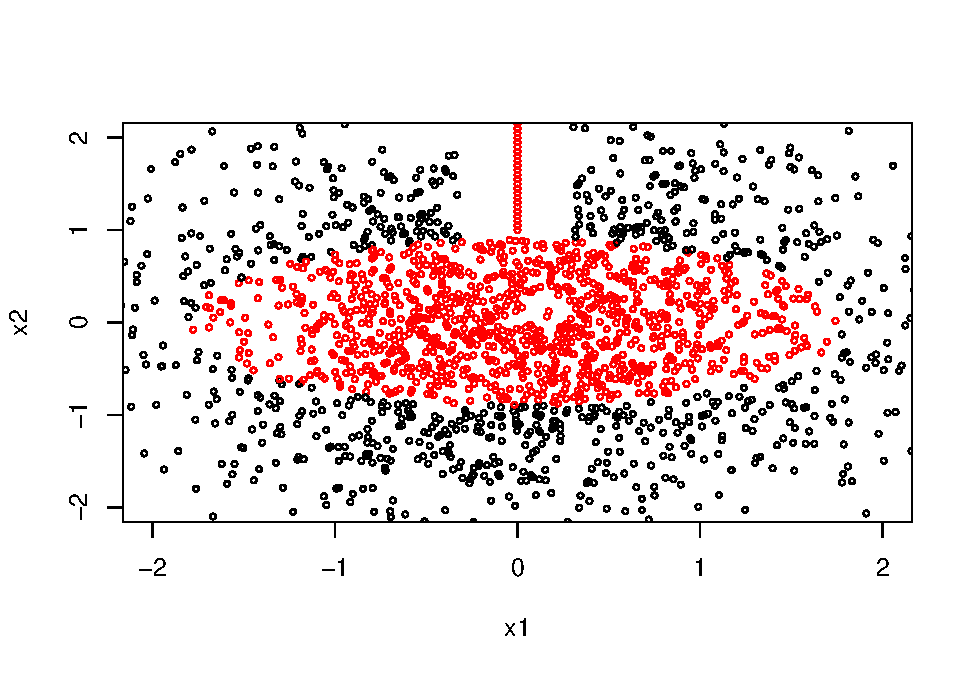
\includegraphics{HW12_files/figure-latex/unnamed-chunk-1-1.pdf}

~

\begin{itemize} \item[(b)]  Let $\eta$ be the parameters of the neural net (i.e. all the $\alpha$'s and $\beta$'s).  What is the dimension of $\eta$ in terms of $m$?  
 
 \ 
 
 \begin{itemize} \item[ ] \hfil \(\displaystyle \dim\left(\eta\right) = m\cdot(2+3)+2 \)


\end{itemize} 
 \end{itemize}

~

\begin{itemize} \item[(c)] Write a function $NN(x, \eta, m)$ which takes a sample $x \in \mathbb{R}^2$ and a choice for $\eta$ and returns the values of $Y_1$ and $Y_2$.  (Hint:  It may be helpful to write functions such as \verb+get_alpha(eta, i)+, which given $\eta$ and $i$ returns $\alpha^{(i)}$,  and \verb+get_alpha_0(eta, i)+, which given $\eta$ and $i$  returns $\alpha^{(i)}_0$.  Using such functions will greatly simplify your code.)
  
 
 \ 
 

 \end{itemize}

\begin{Shaded}
\begin{Highlighting}[]
\NormalTok{X<-}\KeywordTok{as.matrix}\NormalTok{(nn[,}\OperatorTok{-}\DecValTok{3}\NormalTok{])}
\end{Highlighting}
\end{Shaded}

\begin{Shaded}
\begin{Highlighting}[]
\NormalTok{sigmoid<-}\ControlFlowTok{function}\NormalTok{(a,w)\{ (}\DecValTok{1}\OperatorTok{+}\KeywordTok{exp}\NormalTok{(}\OperatorTok{-}\NormalTok{a[}\DecValTok{1}\NormalTok{]}\OperatorTok{-}\KeywordTok{apply}\NormalTok{(w,}\DecValTok{1}\NormalTok{, }\ControlFlowTok{function}\NormalTok{(w)  }\KeywordTok{t}\NormalTok{(a[}\OperatorTok{-}\DecValTok{1}\NormalTok{])}\OperatorTok\NormalTok{w ) ))}\OperatorTok{^}\NormalTok{(}\OperatorTok{-}\DecValTok{1}\NormalTok{)\}}

\NormalTok{NN<-}\ControlFlowTok{function}\NormalTok{(x,eta,m)\{}
    
\NormalTok{    X<-}\KeywordTok{as.matrix}\NormalTok{(x)}

\NormalTok{    Alpha<-}\KeywordTok{matrix}\NormalTok{(eta[}\DecValTok{1}\OperatorTok{:}\KeywordTok{prod}\NormalTok{( }\KeywordTok{c}\NormalTok{(}\KeywordTok{dim}\NormalTok{(X)[}\DecValTok{2}\NormalTok{] }\OperatorTok{+}\StringTok{ }\DecValTok{1}\NormalTok{, m ) )], }\KeywordTok{dim}\NormalTok{(X)[}\DecValTok{2}\NormalTok{] }\OperatorTok{+}\StringTok{ }\DecValTok{1}\NormalTok{ , m)}
\NormalTok{    Z<-}\KeywordTok{apply}\NormalTok{(Alpha,}\DecValTok{2}\NormalTok{, }\ControlFlowTok{function}\NormalTok{(v) }\KeywordTok{sigmoid}\NormalTok{(v,X))}

\NormalTok{    Beta<-}\KeywordTok{matrix}\NormalTok{( eta[(}\KeywordTok{prod}\NormalTok{(}\KeywordTok{dim}\NormalTok{(Alpha))}\OperatorTok{+}\DecValTok{1}\NormalTok{)}\OperatorTok{:}\KeywordTok{length}\NormalTok{(eta) ], }\KeywordTok{dim}\NormalTok{(Z)[}\DecValTok{2}\NormalTok{]}\OperatorTok{+}\DecValTok{1}\NormalTok{, }\DecValTok{2}\NormalTok{)}
     
\NormalTok{    T<-}\KeywordTok{apply}\NormalTok{(Beta,}\DecValTok{2}\NormalTok{, }\ControlFlowTok{function}\NormalTok{(v) }\KeywordTok{sigmoid}\NormalTok{(v,Z))}
\NormalTok{    Y<-}\StringTok{ }\KeywordTok{apply}\NormalTok{(T,}\DecValTok{2}\NormalTok{, }\ControlFlowTok{function}\NormalTok{(x) }\KeywordTok{exp}\NormalTok{(x))}
\NormalTok{    Y<-Y}\OperatorTok{/}\KeywordTok{rowSums}\NormalTok{(Y)}
    \KeywordTok{return}\NormalTok{(Y)}
\NormalTok{\}}

\CommentTok{#test}
\KeywordTok{head}\NormalTok{( }\KeywordTok{NN}\NormalTok{(nn[,}\OperatorTok{-}\DecValTok{3}\NormalTok{],  }\KeywordTok{runif}\NormalTok{(}\DecValTok{22}\NormalTok{,}\OperatorTok{-}\DecValTok{1}\NormalTok{,}\DecValTok{1}\NormalTok{) , }\DecValTok{4}\NormalTok{) )}
\end{Highlighting}
\end{Shaded}

\begin{verbatim}
##           [,1]      [,2]
## [1,] 0.4408756 0.5591244
## [2,] 0.4006250 0.5993750
## [3,] 0.4589122 0.5410878
## [4,] 0.4104487 0.5895513
## [5,] 0.4230657 0.5769343
## [6,] 0.4510645 0.5489355
\end{verbatim}

~

\begin{itemize} \item[(d)] Explain why the log likelihood function $\log L(\eta)$ for the neural net  is given by
\begin{equation}
\log L(\eta) = \sum_{i=1}^N (1-y_i) \log(Y_1) + y_i \log(Y_2).
\end{equation}
(In class, when I wrote the log likelihood, I forgot the log on the $Y_1$ and $Y_2$!)   Write a function that computes $\log L(\eta)$ (you will need to pass the data to the function).  Write a function that uses finite difference to compute the gradient of $\log L(\eta)$.
  
 
 \ 
 
 \begin{itemize} \item[ ]  We are trying to classify each data point by a function that approximates $P(Y|X)$. This is similar to logistic (or other binary regression) because we have two classes and we can derive the likelihood in the same way. Let $\pi = P(y=1|x)$.
 
 \begin{align*}
 \mathcal{L}(\eta) &= \prod_{i=1}^N \pi_i^{y_i} (1-\pi_i)^{1-y_i} \\
 \ell(\eta) &= \sum_{i=1}^N y_i \log(\pi_i) + (1-y_i) \log(1-\pi_i).
 \end{align*}
 
For our neural net, we know our $Y_1 \sim P(y=0|x)$ and $Y_2 \sim P(y=1|x)$, so:

 \begin{align*}
 \ell(\eta) &= \sum_{i=1}^N  (1-y_i) \log(1-\pi_i) + y_i \log(\pi_i) \\
 &= \sum_{i=1}^N    (1-y_i) \log(Y_1) + y_i \log(Y_2).
 \end{align*}
 
\ 


We look at our $ith$ data sample and it can be in one of two classes, $y=0$ or $y=1$. If the sample is of class 0 and the prediction for its probability is $Y_1$, and if it is of class 1 the prediction for its probability is $Y_2$. In the case of neural nets $Y_1$ and $Y_2$ are nested functions that depend on $\eta$ and $x_i$.

\ 

\end{itemize} 
 \end{itemize}

\begin{Shaded}
\begin{Highlighting}[]
\NormalTok{gradL<-}\ControlFlowTok{function}\NormalTok{(eta,x,y,m )\{}
        
\NormalTok{    y<-}\KeywordTok{as.matrix}\NormalTok{(y)}
\NormalTok{    dimeta<-m}\OperatorTok{*}\NormalTok{(}\KeywordTok{dim}\NormalTok{(x)[}\DecValTok{2}\NormalTok{]}\OperatorTok{+}\DecValTok{1}\NormalTok{)}\OperatorTok{+}\DecValTok{2}\OperatorTok{*}\NormalTok{(}\DecValTok{1}\OperatorTok{+}\NormalTok{m)}
\NormalTok{    gradf<-}\KeywordTok{rep}\NormalTok{(}\OtherTok{NA}\NormalTok{,dimeta)}

\NormalTok{    Y<-}\KeywordTok{NN}\NormalTok{(x,eta,m)}
\NormalTok{    ETA<-eta}

\NormalTok{    logl<-}\KeywordTok{sum}\NormalTok{( (}\DecValTok{1}\OperatorTok{-}\NormalTok{y)}\OperatorTok{*}\KeywordTok{log}\NormalTok{(Y[,}\DecValTok{1}\NormalTok{]) }\OperatorTok{+}\StringTok{ }\NormalTok{( y)}\OperatorTok{*}\KeywordTok{log}\NormalTok{(Y[,}\DecValTok{2}\NormalTok{])  )}
    \ControlFlowTok{for}\NormalTok{( i }\ControlFlowTok{in} \DecValTok{1}\OperatorTok{:}\NormalTok{dimeta)\{}
        
\NormalTok{        ETA[i]<-eta[i]}\OperatorTok{+}\NormalTok{(}\DecValTok{10}\OperatorTok{^-}\DecValTok{6}\NormalTok{)}
            
\NormalTok{        Yp<-}\KeywordTok{NN}\NormalTok{(x,ETA,m)}
        
        \CommentTok{#finite difference}
\NormalTok{        gradf[i]<-(}\KeywordTok{sum}\NormalTok{( (}\DecValTok{1}\OperatorTok{-}\NormalTok{y)}\OperatorTok{*}\KeywordTok{log}\NormalTok{(Yp[,}\DecValTok{1}\NormalTok{]) }\OperatorTok{+}\StringTok{ }\NormalTok{( y)}\OperatorTok{*}\KeywordTok{log}\NormalTok{(Yp[,}\DecValTok{2}\NormalTok{])  ) }\OperatorTok{-}\StringTok{ }\NormalTok{logl  ) }\OperatorTok{/}\StringTok{ }\NormalTok{(}\DecValTok{10}\OperatorTok{^-}\DecValTok{6}\NormalTok{) \}}
    
    \KeywordTok{return}\NormalTok{(gradf)}
\NormalTok{\}}

\CommentTok{#test}
\KeywordTok{gradL}\NormalTok{(}\KeywordTok{runif}\NormalTok{(}\DecValTok{22}\NormalTok{,}\OperatorTok{-}\DecValTok{1}\NormalTok{,}\DecValTok{1}\NormalTok{),nn[,}\OperatorTok{-}\DecValTok{3}\NormalTok{],nn[,}\DecValTok{3}\NormalTok{],}\DecValTok{4}\NormalTok{)}
\end{Highlighting}
\end{Shaded}

\begin{verbatim}
##  [1]   -0.9456560   -1.0015087   -0.9444468   -4.3411085   -4.9030621
##  [6]   -8.0070340   12.5980005   13.8016385   15.6020940   14.7172545
## [11]   14.6575887   14.5285653  -27.8164180  -55.4385172  -89.8475744
## [16] -112.9185891 -131.8440047  -89.1537602  -61.4597725  -26.7365051
## [21]   -3.6270790   15.2889804
\end{verbatim}

~

\begin{itemize} \item[(e)] Set $m=4$ and train your neural net by maximizing the $\log L(\eta)$ using steepest ascent.  (It took me roughly $45$ minutes of run time to get a good fit,  roughly $3000$ iterations.  Your results may vary from this depending on implemenation and hardware.)


 
 \ 
 
 \end{itemize}

\begin{Shaded}
\begin{Highlighting}[]
\NormalTok{logL<-}\ControlFlowTok{function}\NormalTok{(x,y,eta,m)\{}
\NormalTok{    Y<-}\KeywordTok{NN}\NormalTok{(x,eta,m)}
    \KeywordTok{return}\NormalTok{( }\KeywordTok{sum}\NormalTok{( (}\DecValTok{1}\OperatorTok{-}\NormalTok{y)}\OperatorTok{*}\KeywordTok{log}\NormalTok{(Y[,}\DecValTok{1}\NormalTok{]) }\OperatorTok{+}\StringTok{ }\NormalTok{( y)}\OperatorTok{*}\KeywordTok{log}\NormalTok{(Y[,}\DecValTok{2}\NormalTok{])  ) )    \}}

\NormalTok{j=}\DecValTok{1}\NormalTok{;current_grad <-}\StringTok{ }\KeywordTok{gradL}\NormalTok{(Alpha , X , nn[,}\DecValTok{3}\NormalTok{] , }\DecValTok{4}\NormalTok{ ) }

\ControlFlowTok{for}\NormalTok{(i }\ControlFlowTok{in}\NormalTok{ j}\OperatorTok{:}\NormalTok{(}\DecValTok{3000}\NormalTok{)) \{}

\NormalTok{    d <-}\StringTok{ }\NormalTok{current_grad}\OperatorTok{/}\KeywordTok{Norm}\NormalTok{(current_grad)    }
    
\NormalTok{    s <-}\StringTok{ }\DecValTok{1} 
\NormalTok{    current_logL <-}\StringTok{ }\KeywordTok{logL}\NormalTok{(X,nn[,}\DecValTok{3}\NormalTok{],Alpha,}\DecValTok{4}\NormalTok{)}

    \ControlFlowTok{while}\NormalTok{(}\KeywordTok{logL}\NormalTok{(X,nn[,}\DecValTok{3}\NormalTok{],Alpha}\OperatorTok{+}\NormalTok{s}\OperatorTok{*}\NormalTok{d,}\DecValTok{4}\NormalTok{)  }\OperatorTok{<}\StringTok{ }\NormalTok{current_logL)}
\NormalTok{         s <-}\StringTok{ }\NormalTok{s}\OperatorTok{/}\DecValTok{2} 

\NormalTok{  Alpha <-}\StringTok{ }\NormalTok{Alpha }\OperatorTok{+}\StringTok{ }\NormalTok{s}\OperatorTok{*}\NormalTok{d}
\NormalTok{  current_grad <-}\StringTok{  }\KeywordTok{gradL}\NormalTok{(Alpha , X , nn[,}\DecValTok{3}\NormalTok{] , }\DecValTok{4}\NormalTok{ ) \}  }
\end{Highlighting}
\end{Shaded}

\begin{Shaded}
\begin{Highlighting}[]
\CommentTok{#Alpha is eta (alphas and betas)}
\NormalTok{Alpha}
\end{Highlighting}
\end{Shaded}

\begin{verbatim}
##  [1]  -3.7748365   2.1178734   0.3139542  -5.5415006  -0.5958018
##  [6]   5.8168459  11.0561352   0.2074085  14.0207743  25.2868297
## [11]  16.0428078   3.8300725  15.9792114  23.4815794  23.2210775
## [16] -13.5097426 -12.2073593 -18.6510642 -27.0546378 -27.4979835
## [21]  15.2350215  14.7081561
\end{verbatim}

\begin{Shaded}
\begin{Highlighting}[]
\KeywordTok{multiplot}\NormalTok{(}\KeywordTok{ggplot}\NormalTok{(test, }\KeywordTok{aes}\NormalTok{(x1, x2)) }\OperatorTok{+}\StringTok{ }\KeywordTok{geom_point}\NormalTok{(}\KeywordTok{aes}\NormalTok{(}\DataTypeTok{colour =} \KeywordTok{factor}\NormalTok{(y3))) }\OperatorTok{+}
\StringTok{            }\KeywordTok{theme}\NormalTok{(}\DataTypeTok{legend.position=}\StringTok{"bottom"}\NormalTok{)}\OperatorTok{+}\StringTok{ }\KeywordTok{ggtitle}\NormalTok{(}\StringTok{"Test"}\NormalTok{)   ,p }\OperatorTok{+}\StringTok{ }\KeywordTok{ggtitle}\NormalTok{(}\StringTok{"Actual"}\NormalTok{) ,  }\DataTypeTok{cols=}\DecValTok{2}\NormalTok{ ) }
\end{Highlighting}
\end{Shaded}

\includegraphics{HW12_files/figure-latex/unnamed-chunk-7-1.pdf}

~

\begin{itemize}\item[]  \hfil Decent fit with a cutoff of $p=0.5$, but it is not overfitting the ``tail'' part.
\end{itemize}

~

\begin{itemize} \item[(f)] Remember that a classifier in this case is a function $F(x) : \mathbb{R}^2 \to \{0, 1\}$, where $x \in \mathbb{R}^2$.   Once you choose $\eta$ by by computing the maximum likelihood in (e), choose a cutoff $p \in [0,1]$.  Set $F$ by
\begin{equation}
F(x) = \big\{
\begin{array}{cc}
0 & \text{if } Y_1(x, \eta) < p \\ 
1 & \text{if } Y_1(x, \eta) \ge p
\end{array}
\end{equation} 
Try different value of $p$ and for each $p$, visualize your classifier.  
 \ 
 
\end{itemize}

\begin{Shaded}
\begin{Highlighting}[]
\NormalTok{x1<-}\KeywordTok{matrix}\NormalTok{(}\DecValTok{4}\OperatorTok{*}\KeywordTok{runif}\NormalTok{(}\DecValTok{20000}\NormalTok{ )}\OperatorTok{-}\DecValTok{2}\NormalTok{, }\DecValTok{10000}\NormalTok{,}\DecValTok{2}\NormalTok{)}
\NormalTok{test<-}\KeywordTok{as.data.frame}\NormalTok{((}\KeywordTok{NN}\NormalTok{(x1,Alpha ,}\DecValTok{4}\NormalTok{)))}
\NormalTok{test<-}\KeywordTok{cbind}\NormalTok{(test,x1)}
\NormalTok{test}\OperatorTok{$}\NormalTok{y1<-}\StringTok{ }\KeywordTok{ifelse}\NormalTok{( test[,}\DecValTok{1}\NormalTok{]}\OperatorTok{>}\NormalTok{.}\DecValTok{5}\NormalTok{ , }\DecValTok{0}\NormalTok{,}\DecValTok{1}\NormalTok{)}
\NormalTok{test}\OperatorTok{$}\NormalTok{y2<-}\StringTok{ }\KeywordTok{ifelse}\NormalTok{( test[,}\DecValTok{1}\NormalTok{]}\OperatorTok{>}\NormalTok{.}\DecValTok{7}\NormalTok{ , }\DecValTok{0}\NormalTok{,}\DecValTok{1}\NormalTok{)}
\NormalTok{test}\OperatorTok{$}\NormalTok{y3<-}\StringTok{ }\KeywordTok{ifelse}\NormalTok{( test[,}\DecValTok{1}\NormalTok{]}\OperatorTok{>}\NormalTok{.}\DecValTok{3}\NormalTok{ , }\DecValTok{0}\NormalTok{,}\DecValTok{1}\NormalTok{)}
\KeywordTok{names}\NormalTok{(test)[}\DecValTok{3}\OperatorTok{:}\DecValTok{4}\NormalTok{]<-}\KeywordTok{c}\NormalTok{(}\StringTok{"x1"}\NormalTok{,}\StringTok{"x2"}\NormalTok{)}

\NormalTok{p1 <-}\StringTok{ }\KeywordTok{ggplot}\NormalTok{(test, }\KeywordTok{aes}\NormalTok{(x1, x2)) }\OperatorTok{+}\StringTok{ }\KeywordTok{geom_point}\NormalTok{(}\KeywordTok{aes}\NormalTok{(}\DataTypeTok{colour =} \KeywordTok{factor}\NormalTok{(y1))) }\OperatorTok{+}
\StringTok{  }\KeywordTok{ylim}\NormalTok{(}\OperatorTok{-}\FloatTok{2.5}\NormalTok{, }\FloatTok{2.5}\NormalTok{) }\OperatorTok{+}\StringTok{ }\KeywordTok{xlim}\NormalTok{( }\OperatorTok{-}\FloatTok{2.5}\NormalTok{,}\FloatTok{2.5}\NormalTok{ ) }\OperatorTok{+}\StringTok{ }\KeywordTok{ggtitle}\NormalTok{(}\StringTok{"p = 0.5"}\NormalTok{) }\OperatorTok{+}
\StringTok{  }\KeywordTok{theme}\NormalTok{(}\DataTypeTok{legend.position=}\StringTok{"bottom"}\NormalTok{)}
\NormalTok{p2 <-}\StringTok{ }\KeywordTok{ggplot}\NormalTok{(test, }\KeywordTok{aes}\NormalTok{(x1, x2)) }\OperatorTok{+}\StringTok{ }\KeywordTok{geom_point}\NormalTok{(}\KeywordTok{aes}\NormalTok{(}\DataTypeTok{colour =} \KeywordTok{factor}\NormalTok{(y2))) }\OperatorTok{+}
\StringTok{  }\KeywordTok{ylim}\NormalTok{(}\OperatorTok{-}\FloatTok{2.5}\NormalTok{, }\FloatTok{2.5}\NormalTok{) }\OperatorTok{+}\StringTok{ }\KeywordTok{xlim}\NormalTok{( }\OperatorTok{-}\FloatTok{2.5}\NormalTok{,}\FloatTok{2.5}\NormalTok{ ) }\OperatorTok{+}\StringTok{ }\KeywordTok{ggtitle}\NormalTok{(}\StringTok{"p = 0.7"}\NormalTok{) }\OperatorTok{+}
\StringTok{  }\KeywordTok{theme}\NormalTok{(}\DataTypeTok{legend.position=}\StringTok{"bottom"}\NormalTok{)}
\NormalTok{p3 <-}\StringTok{ }\KeywordTok{ggplot}\NormalTok{(test, }\KeywordTok{aes}\NormalTok{(x1, x2)) }\OperatorTok{+}\StringTok{ }\KeywordTok{geom_point}\NormalTok{(}\KeywordTok{aes}\NormalTok{(}\DataTypeTok{colour =} \KeywordTok{factor}\NormalTok{(y3))) }\OperatorTok{+}
\StringTok{  }\KeywordTok{ylim}\NormalTok{(}\OperatorTok{-}\FloatTok{2.5}\NormalTok{, }\FloatTok{2.5}\NormalTok{) }\OperatorTok{+}\StringTok{ }\KeywordTok{xlim}\NormalTok{( }\OperatorTok{-}\FloatTok{2.5}\NormalTok{,}\FloatTok{2.5}\NormalTok{ ) }\OperatorTok{+}\StringTok{ }\KeywordTok{ggtitle}\NormalTok{(}\StringTok{"p = 0.3"}\NormalTok{) }\OperatorTok{+}
\StringTok{  }\KeywordTok{theme}\NormalTok{(}\DataTypeTok{legend.position=}\StringTok{"bottom"}\NormalTok{)}
\NormalTok{p<-}\StringTok{ }\NormalTok{p }\OperatorTok{+}\StringTok{ }\KeywordTok{ggtitle}\NormalTok{(}\StringTok{"original data"}\NormalTok{) }
\KeywordTok{multiplot}\NormalTok{(p1, p2, p3,p,  }\DataTypeTok{cols=}\DecValTok{2}\NormalTok{)}
\end{Highlighting}
\end{Shaded}

\includegraphics{HW12_files/figure-latex/unnamed-chunk-8-1.pdf}

~

\newpage

\begin{itemize} \item[(g)] Now repeat (e) and (f), but in your log likelihood, include a penalty term of the form,

\ 


\begin{equation}
\rho \left(\sum_{i=1}^m \|\alpha^{(i)}\|^2 + \sum_{j=1}^2 \|\beta^{(j)}\|^2\right).
\end{equation}

\ 


Given that we are maximizing, explain why you should subtract the penalty term rather than add it onto the log-likelihood in (d).
Train your net with several values of $\rho$, visualize the resulting classifier for differnt $p$, and compare your results.


 \ 
 
 \begin{itemize} \item[] We wish to maximize the likelihood (or alternatively the log-likelihood) so in order to impose a penalty we will reduce the likelihood. This is done by subtracting the penalty term rather than adding it.

 
\end{itemize} 
\end{itemize}

~

\begin{Shaded}
\begin{Highlighting}[]
\CommentTok{#Penalized Log likelihood function}
\NormalTok{PlogL<-}\ControlFlowTok{function}\NormalTok{(x,y,eta,m,rho)\{}
\NormalTok{    X<-}\KeywordTok{as.matrix}\NormalTok{(x)}
\NormalTok{    ALPHA<-}\KeywordTok{matrix}\NormalTok{(eta[}\DecValTok{1}\OperatorTok{:}\KeywordTok{prod}\NormalTok{( }\KeywordTok{c}\NormalTok{(}\KeywordTok{dim}\NormalTok{(X)[}\DecValTok{2}\NormalTok{] }\OperatorTok{+}\StringTok{ }\DecValTok{1}\NormalTok{, m ) )], }\KeywordTok{dim}\NormalTok{(X)[}\DecValTok{2}\NormalTok{] }\OperatorTok{+}\StringTok{ }\DecValTok{1}\NormalTok{ , m)}
\NormalTok{    Beta<-}\KeywordTok{matrix}\NormalTok{(eta[(}\KeywordTok{prod}\NormalTok{( }\KeywordTok{c}\NormalTok{(}\KeywordTok{dim}\NormalTok{(X)[}\DecValTok{2}\NormalTok{] }\OperatorTok{+}\StringTok{ }\DecValTok{1}\NormalTok{, m ) )}\OperatorTok{+}\DecValTok{1}\NormalTok{)}\OperatorTok{:}\KeywordTok{length}\NormalTok{(eta)],}
\NormalTok{        m}\OperatorTok{+}\DecValTok{1}\NormalTok{,}\DecValTok{2}\NormalTok{)}
\NormalTok{    ALPHA<-}\KeywordTok{as.vector}\NormalTok{(}\KeywordTok{t}\NormalTok{(ALPHA[}\OperatorTok{-}\DecValTok{1}\NormalTok{ ,])) ;Beta<-}\KeywordTok{as.vector}\NormalTok{(}\KeywordTok{t}\NormalTok{(Beta[}\OperatorTok{-}\DecValTok{1}\NormalTok{ ,]))}
\NormalTok{  Norm <-}\StringTok{ }\ControlFlowTok{function}\NormalTok{(w)\{  }\KeywordTok{sqrt}\NormalTok{(}\KeywordTok{sum}\NormalTok{(w}\OperatorTok{^}\DecValTok{2}\NormalTok{))\}}

\NormalTok{    Y<-}\KeywordTok{NN}\NormalTok{(x,eta,m)}
    \KeywordTok{return}\NormalTok{( }\KeywordTok{sum}\NormalTok{( (}\DecValTok{1}\OperatorTok{-}\NormalTok{y)}\OperatorTok{*}\KeywordTok{log}\NormalTok{(Y[,}\DecValTok{1}\NormalTok{]) }\OperatorTok{+}\StringTok{ }\NormalTok{( y)}\OperatorTok{*}\KeywordTok{log}\NormalTok{(Y[,}\DecValTok{2}\NormalTok{])  ) }\OperatorTok{-}
\StringTok{        }\NormalTok{rho}\OperatorTok{*}\NormalTok{(}\KeywordTok{sum}\NormalTok{(}\KeywordTok{Norm}\NormalTok{(ALPHA)}\OperatorTok{^}\DecValTok{2}\NormalTok{)}\OperatorTok{+}\KeywordTok{sum}\NormalTok{(}\KeywordTok{Norm}\NormalTok{(Beta)}\OperatorTok{^}\DecValTok{2}\NormalTok{) )}
\NormalTok{    )   \}}
\end{Highlighting}
\end{Shaded}

~

\hfil {\Large $\rho = 0.1$}

~

\begin{Shaded}
\begin{Highlighting}[]
\NormalTok{j=}\DecValTok{1}\NormalTok{;current_grad <-}\StringTok{ }\KeywordTok{gradL}\NormalTok{(Alpha , X , nn[,}\DecValTok{3}\NormalTok{] , }\DecValTok{4}\NormalTok{ ) }
\KeywordTok{system.time}\NormalTok{(}
 \ControlFlowTok{for}\NormalTok{(i }\ControlFlowTok{in}\NormalTok{ j}\OperatorTok{:}\NormalTok{(}\DecValTok{2000}\NormalTok{)) \{}
    \CommentTok{#iter <- iter + 1}
    
\NormalTok{    d <-}\StringTok{ }\NormalTok{current_grad}\OperatorTok{/}\KeywordTok{Norm}\NormalTok{(current_grad)    }
    
\NormalTok{    s <-}\StringTok{ }\DecValTok{1} 
    \CommentTok{#Penalized Log likelihood}
\NormalTok{    current_logL <-}\StringTok{ }\KeywordTok{PlogL}\NormalTok{(X,nn[,}\DecValTok{3}\NormalTok{],Alpha,}\DecValTok{4}\NormalTok{,.}\DecValTok{1}\NormalTok{)}
    
    \ControlFlowTok{while}\NormalTok{(}\KeywordTok{logL}\NormalTok{(X,nn[,}\DecValTok{3}\NormalTok{],Alpha}\OperatorTok{+}\NormalTok{s}\OperatorTok{*}\NormalTok{d,}\DecValTok{4}\NormalTok{)  }\OperatorTok{<}\StringTok{ }\NormalTok{current_logL)}
\NormalTok{         s <-}\StringTok{ }\NormalTok{s}\OperatorTok{/}\DecValTok{2} 

\NormalTok{    Alpha <-}\StringTok{ }\NormalTok{Alpha }\OperatorTok{+}\StringTok{ }\NormalTok{s}\OperatorTok{*}\NormalTok{d}
\NormalTok{    current_grad <-}\StringTok{  }\KeywordTok{gradL}\NormalTok{(Alpha , X , nn[,}\DecValTok{3}\NormalTok{] , }\DecValTok{4}\NormalTok{ ) \} )}


\NormalTok{j=i}
\end{Highlighting}
\end{Shaded}

\begin{verbatim}
##  [1]  -4.217173   2.129696   2.291096  -5.749465  -1.505578   5.422963
##  [7]  10.917247  -2.730573  12.886107  10.326642   5.094741   9.110171
## [13]  13.503592  21.919573  22.305991 -10.991376 -10.851156 -14.688772
## [19] -23.092542 -24.351591  12.003044  12.654236
\end{verbatim}

\begin{Shaded}
\begin{Highlighting}[]
\NormalTok{x1<-}\KeywordTok{matrix}\NormalTok{(}\DecValTok{4}\OperatorTok{*}\KeywordTok{runif}\NormalTok{(}\DecValTok{10000}\NormalTok{ )}\OperatorTok{-}\DecValTok{2}\NormalTok{, }\DecValTok{5000}\NormalTok{,}\DecValTok{2}\NormalTok{)}
\NormalTok{test<-}\KeywordTok{as.data.frame}\NormalTok{((}\KeywordTok{NN}\NormalTok{(x1,Alpha ,}\DecValTok{4}\NormalTok{)))}
\NormalTok{test<-}\KeywordTok{cbind}\NormalTok{(test,x1)}
\NormalTok{test}\OperatorTok{$}\NormalTok{y1<-}\StringTok{ }\KeywordTok{ifelse}\NormalTok{( test[,}\DecValTok{1}\NormalTok{]}\OperatorTok{>}\NormalTok{.}\DecValTok{5}\NormalTok{ , }\DecValTok{0}\NormalTok{,}\DecValTok{1}\NormalTok{)}
\NormalTok{test}\OperatorTok{$}\NormalTok{y2<-}\StringTok{ }\KeywordTok{ifelse}\NormalTok{( test[,}\DecValTok{1}\NormalTok{]}\OperatorTok{>}\NormalTok{.}\DecValTok{7}\NormalTok{ , }\DecValTok{0}\NormalTok{,}\DecValTok{1}\NormalTok{)}
\NormalTok{test}\OperatorTok{$}\NormalTok{y3<-}\StringTok{ }\KeywordTok{ifelse}\NormalTok{( test[,}\DecValTok{1}\NormalTok{]}\OperatorTok{>}\NormalTok{.}\DecValTok{3}\NormalTok{ , }\DecValTok{0}\NormalTok{,}\DecValTok{1}\NormalTok{)}
\KeywordTok{names}\NormalTok{(test)[}\DecValTok{3}\OperatorTok{:}\DecValTok{4}\NormalTok{]<-}\KeywordTok{c}\NormalTok{(}\StringTok{"x1"}\NormalTok{,}\StringTok{"x2"}\NormalTok{)}

\NormalTok{p1 <-}\StringTok{ }\KeywordTok{ggplot}\NormalTok{(test, }\KeywordTok{aes}\NormalTok{(x1, x2)) }\OperatorTok{+}\StringTok{ }\KeywordTok{geom_point}\NormalTok{(}\KeywordTok{aes}\NormalTok{(}\DataTypeTok{colour =} \KeywordTok{factor}\NormalTok{(y1))) }\OperatorTok{+}
\StringTok{  }\KeywordTok{ylim}\NormalTok{(}\OperatorTok{-}\FloatTok{2.5}\NormalTok{, }\FloatTok{2.5}\NormalTok{) }\OperatorTok{+}\StringTok{ }\KeywordTok{xlim}\NormalTok{( }\OperatorTok{-}\FloatTok{2.5}\NormalTok{,}\FloatTok{2.5}\NormalTok{ ) }\OperatorTok{+}\StringTok{ }\KeywordTok{ggtitle}\NormalTok{(}\StringTok{"p = 0.5"}\NormalTok{) }\OperatorTok{+}
\StringTok{  }\KeywordTok{theme}\NormalTok{(}\DataTypeTok{legend.position=}\StringTok{"bottom"}\NormalTok{)}
\NormalTok{p2 <-}\StringTok{ }\KeywordTok{ggplot}\NormalTok{(test, }\KeywordTok{aes}\NormalTok{(x1, x2)) }\OperatorTok{+}\StringTok{ }\KeywordTok{geom_point}\NormalTok{(}\KeywordTok{aes}\NormalTok{(}\DataTypeTok{colour =} \KeywordTok{factor}\NormalTok{(y2))) }\OperatorTok{+}
\StringTok{  }\KeywordTok{ylim}\NormalTok{(}\OperatorTok{-}\FloatTok{2.5}\NormalTok{, }\FloatTok{2.5}\NormalTok{) }\OperatorTok{+}\StringTok{ }\KeywordTok{xlim}\NormalTok{( }\OperatorTok{-}\FloatTok{2.5}\NormalTok{,}\FloatTok{2.5}\NormalTok{ ) }\OperatorTok{+}\StringTok{ }\KeywordTok{ggtitle}\NormalTok{(}\StringTok{"p = 0.7"}\NormalTok{) }\OperatorTok{+}
\StringTok{  }\KeywordTok{theme}\NormalTok{(}\DataTypeTok{legend.position=}\StringTok{"bottom"}\NormalTok{)}
\NormalTok{p3 <-}\StringTok{ }\KeywordTok{ggplot}\NormalTok{(test, }\KeywordTok{aes}\NormalTok{(x1, x2)) }\OperatorTok{+}\StringTok{ }\KeywordTok{geom_point}\NormalTok{(}\KeywordTok{aes}\NormalTok{(}\DataTypeTok{colour =} \KeywordTok{factor}\NormalTok{(y3))) }\OperatorTok{+}
\StringTok{  }\KeywordTok{ylim}\NormalTok{(}\OperatorTok{-}\FloatTok{2.5}\NormalTok{, }\FloatTok{2.5}\NormalTok{) }\OperatorTok{+}\StringTok{ }\KeywordTok{xlim}\NormalTok{( }\OperatorTok{-}\FloatTok{2.5}\NormalTok{,}\FloatTok{2.5}\NormalTok{ ) }\OperatorTok{+}\StringTok{ }\KeywordTok{ggtitle}\NormalTok{(}\StringTok{"p = 0.3"}\NormalTok{) }\OperatorTok{+}
\StringTok{  }\KeywordTok{theme}\NormalTok{(}\DataTypeTok{legend.position=}\StringTok{"bottom"}\NormalTok{)}

\KeywordTok{multiplot}\NormalTok{(p1, p2, p3,  p,}\DataTypeTok{cols=}\DecValTok{2}\NormalTok{)}
\end{Highlighting}
\end{Shaded}

\includegraphics{HW12_files/figure-latex/unnamed-chunk-12-1.pdf}

~

\hfil {\Large $\rho = 1$}

~

\begin{Shaded}
\begin{Highlighting}[]
\NormalTok{j=}\DecValTok{1}\NormalTok{;current_grad <-}\StringTok{ }\KeywordTok{gradL}\NormalTok{(Alpha , X , nn[,}\DecValTok{3}\NormalTok{] , }\DecValTok{4}\NormalTok{ ) }
\KeywordTok{system.time}\NormalTok{(}
 \ControlFlowTok{for}\NormalTok{(i }\ControlFlowTok{in}\NormalTok{ j}\OperatorTok{:}\NormalTok{(}\DecValTok{2000}\NormalTok{)) \{}
    \CommentTok{#iter <- iter + 1}
    
\NormalTok{    d <-}\StringTok{ }\NormalTok{current_grad}\OperatorTok{/}\KeywordTok{Norm}\NormalTok{(current_grad)    }
    
\NormalTok{    s <-}\StringTok{ }\DecValTok{1} 
\NormalTok{    current_logL <-}\StringTok{ }\KeywordTok{PlogL}\NormalTok{(X,nn[,}\DecValTok{3}\NormalTok{],Alpha,}\DecValTok{4}\NormalTok{,}\DecValTok{1}\NormalTok{)}
    
    \ControlFlowTok{while}\NormalTok{(}\KeywordTok{logL}\NormalTok{(X,nn[,}\DecValTok{3}\NormalTok{],Alpha}\OperatorTok{+}\NormalTok{s}\OperatorTok{*}\NormalTok{d,}\DecValTok{4}\NormalTok{)  }\OperatorTok{<}\StringTok{ }\NormalTok{current_logL)}
\NormalTok{         s <-}\StringTok{ }\NormalTok{s}\OperatorTok{/}\DecValTok{2} 

\NormalTok{    Alpha <-}\StringTok{ }\NormalTok{Alpha }\OperatorTok{+}\StringTok{ }\NormalTok{s}\OperatorTok{*}\NormalTok{d}
\NormalTok{    current_grad <-}\StringTok{  }\KeywordTok{gradL}\NormalTok{(Alpha , X , nn[,}\DecValTok{3}\NormalTok{] , }\DecValTok{4}\NormalTok{ ) \} )}


\NormalTok{j=i}
\end{Highlighting}
\end{Shaded}

~

\begin{verbatim}
##  [1]  -5.012726   2.095720   3.540725  -5.324588  -2.108554   3.957979
##  [7]   9.760088  -4.196175   9.938802   6.688340   2.643233   7.210336
## [13]  15.743670  24.279396  24.855088 -12.204780 -14.039753 -18.199320
## [19] -26.719915 -28.098740  13.621660  15.881839
\end{verbatim}

\begin{Shaded}
\begin{Highlighting}[]
\NormalTok{x1<-}\KeywordTok{matrix}\NormalTok{(}\DecValTok{4}\OperatorTok{*}\KeywordTok{runif}\NormalTok{(}\DecValTok{10000}\NormalTok{ )}\OperatorTok{-}\DecValTok{2}\NormalTok{, }\DecValTok{5000}\NormalTok{,}\DecValTok{2}\NormalTok{)}
\NormalTok{test<-}\KeywordTok{as.data.frame}\NormalTok{((}\KeywordTok{NN}\NormalTok{(x1,Alpha ,}\DecValTok{4}\NormalTok{)))}
\NormalTok{test<-}\KeywordTok{cbind}\NormalTok{(test,x1)}
\NormalTok{test}\OperatorTok{$}\NormalTok{y1<-}\StringTok{ }\KeywordTok{ifelse}\NormalTok{( test[,}\DecValTok{1}\NormalTok{]}\OperatorTok{>}\NormalTok{.}\DecValTok{5}\NormalTok{ , }\DecValTok{0}\NormalTok{,}\DecValTok{1}\NormalTok{)}
\NormalTok{test}\OperatorTok{$}\NormalTok{y2<-}\StringTok{ }\KeywordTok{ifelse}\NormalTok{( test[,}\DecValTok{1}\NormalTok{]}\OperatorTok{>}\NormalTok{.}\DecValTok{7}\NormalTok{ , }\DecValTok{0}\NormalTok{,}\DecValTok{1}\NormalTok{)}
\NormalTok{test}\OperatorTok{$}\NormalTok{y3<-}\StringTok{ }\KeywordTok{ifelse}\NormalTok{( test[,}\DecValTok{1}\NormalTok{]}\OperatorTok{>}\NormalTok{.}\DecValTok{3}\NormalTok{ , }\DecValTok{0}\NormalTok{,}\DecValTok{1}\NormalTok{)}
\KeywordTok{names}\NormalTok{(test)[}\DecValTok{3}\OperatorTok{:}\DecValTok{4}\NormalTok{]<-}\KeywordTok{c}\NormalTok{(}\StringTok{"x1"}\NormalTok{,}\StringTok{"x2"}\NormalTok{)}

\NormalTok{p1 <-}\StringTok{ }\KeywordTok{ggplot}\NormalTok{(test, }\KeywordTok{aes}\NormalTok{(x1, x2)) }\OperatorTok{+}\StringTok{ }\KeywordTok{geom_point}\NormalTok{(}\KeywordTok{aes}\NormalTok{(}\DataTypeTok{colour =} \KeywordTok{factor}\NormalTok{(y1))) }\OperatorTok{+}
\StringTok{  }\KeywordTok{ylim}\NormalTok{(}\OperatorTok{-}\FloatTok{2.5}\NormalTok{, }\FloatTok{2.5}\NormalTok{) }\OperatorTok{+}\StringTok{ }\KeywordTok{xlim}\NormalTok{( }\OperatorTok{-}\FloatTok{2.5}\NormalTok{,}\FloatTok{2.5}\NormalTok{ ) }\OperatorTok{+}\StringTok{ }\KeywordTok{ggtitle}\NormalTok{(}\StringTok{"p = 0.5"}\NormalTok{) }\OperatorTok{+}
\StringTok{  }\KeywordTok{theme}\NormalTok{(}\DataTypeTok{legend.position=}\StringTok{"bottom"}\NormalTok{)}
\NormalTok{p2 <-}\StringTok{ }\KeywordTok{ggplot}\NormalTok{(test, }\KeywordTok{aes}\NormalTok{(x1, x2)) }\OperatorTok{+}\StringTok{ }\KeywordTok{geom_point}\NormalTok{(}\KeywordTok{aes}\NormalTok{(}\DataTypeTok{colour =} \KeywordTok{factor}\NormalTok{(y2))) }\OperatorTok{+}
\StringTok{  }\KeywordTok{ylim}\NormalTok{(}\OperatorTok{-}\FloatTok{2.5}\NormalTok{, }\FloatTok{2.5}\NormalTok{) }\OperatorTok{+}\StringTok{ }\KeywordTok{xlim}\NormalTok{( }\OperatorTok{-}\FloatTok{2.5}\NormalTok{,}\FloatTok{2.5}\NormalTok{ ) }\OperatorTok{+}\StringTok{ }\KeywordTok{ggtitle}\NormalTok{(}\StringTok{"p = 0.7"}\NormalTok{) }\OperatorTok{+}
\StringTok{  }\KeywordTok{theme}\NormalTok{(}\DataTypeTok{legend.position=}\StringTok{"bottom"}\NormalTok{)}
\NormalTok{p3 <-}\StringTok{ }\KeywordTok{ggplot}\NormalTok{(test, }\KeywordTok{aes}\NormalTok{(x1, x2)) }\OperatorTok{+}\StringTok{ }\KeywordTok{geom_point}\NormalTok{(}\KeywordTok{aes}\NormalTok{(}\DataTypeTok{colour =} \KeywordTok{factor}\NormalTok{(y3))) }\OperatorTok{+}
\StringTok{  }\KeywordTok{ylim}\NormalTok{(}\OperatorTok{-}\FloatTok{2.5}\NormalTok{, }\FloatTok{2.5}\NormalTok{) }\OperatorTok{+}\StringTok{ }\KeywordTok{xlim}\NormalTok{( }\OperatorTok{-}\FloatTok{2.5}\NormalTok{,}\FloatTok{2.5}\NormalTok{ ) }\OperatorTok{+}\StringTok{ }\KeywordTok{ggtitle}\NormalTok{(}\StringTok{"p = 0.3"}\NormalTok{) }\OperatorTok{+}
\StringTok{  }\KeywordTok{theme}\NormalTok{(}\DataTypeTok{legend.position=}\StringTok{"bottom"}\NormalTok{)}

\KeywordTok{multiplot}\NormalTok{(p1, p2, p3,  p, }\DataTypeTok{cols=}\DecValTok{2}\NormalTok{)}
\end{Highlighting}
\end{Shaded}

\includegraphics{HW12_files/figure-latex/unnamed-chunk-15-1.pdf}

\hfil {\Large $\rho = 100$}

~

\begin{Shaded}
\begin{Highlighting}[]
\NormalTok{j=}\DecValTok{1}\NormalTok{;current_grad <-}\StringTok{ }\KeywordTok{gradL}\NormalTok{(Alpha , X , nn[,}\DecValTok{3}\NormalTok{] , }\DecValTok{4}\NormalTok{ ) }
\KeywordTok{system.time}\NormalTok{(}
 \ControlFlowTok{for}\NormalTok{(i }\ControlFlowTok{in}\NormalTok{ j}\OperatorTok{:}\NormalTok{(}\DecValTok{2000}\NormalTok{)) \{}

\NormalTok{    d <-}\StringTok{ }\NormalTok{current_grad}\OperatorTok{/}\KeywordTok{Norm}\NormalTok{(current_grad)    }
    
\NormalTok{    s <-}\StringTok{ }\DecValTok{1} 
\NormalTok{    current_logL <-}\StringTok{ }\KeywordTok{PlogL}\NormalTok{(X,nn[,}\DecValTok{3}\NormalTok{],Alpha,}\DecValTok{4}\NormalTok{,}\DecValTok{100}\NormalTok{)}
    
    \ControlFlowTok{while}\NormalTok{(}\KeywordTok{logL}\NormalTok{(X,nn[,}\DecValTok{3}\NormalTok{],Alpha}\OperatorTok{+}\NormalTok{s}\OperatorTok{*}\NormalTok{d,}\DecValTok{4}\NormalTok{)  }\OperatorTok{<}\StringTok{ }\NormalTok{current_logL)}
\NormalTok{         s <-}\StringTok{ }\NormalTok{s}\OperatorTok{/}\DecValTok{2} 

\NormalTok{    Alpha <-}\StringTok{ }\NormalTok{Alpha }\OperatorTok{+}\StringTok{ }\NormalTok{s}\OperatorTok{*}\NormalTok{d}
\NormalTok{    current_grad <-}\StringTok{  }\KeywordTok{gradL}\NormalTok{(Alpha , X , nn[,}\DecValTok{3}\NormalTok{] , }\DecValTok{4}\NormalTok{ ) \} )}


\NormalTok{j=i}
\end{Highlighting}
\end{Shaded}

~

\begin{verbatim}
##  [1]  -4.80870303   2.51425207  -0.70430171  -8.39809328   0.07027287
##  [6]   8.89975250  13.39129423   0.16705617  16.70429985  19.56583078
## [11]  10.80716806  10.69527465  12.34268115  20.81992539  21.16594983
## [16]  -9.72328246 -10.27706135 -12.66218131 -21.14339824 -22.67591064
## [21]   9.49389847  10.38622987
\end{verbatim}

\begin{Shaded}
\begin{Highlighting}[]
\NormalTok{x1<-}\KeywordTok{matrix}\NormalTok{(}\DecValTok{4}\OperatorTok{*}\KeywordTok{runif}\NormalTok{(}\DecValTok{10000}\NormalTok{ )}\OperatorTok{-}\DecValTok{2}\NormalTok{, }\DecValTok{5000}\NormalTok{,}\DecValTok{2}\NormalTok{)}
\NormalTok{test<-}\KeywordTok{as.data.frame}\NormalTok{((}\KeywordTok{NN}\NormalTok{(x1,Alpha ,}\DecValTok{4}\NormalTok{)))}
\NormalTok{test<-}\KeywordTok{cbind}\NormalTok{(test,x1)}
\NormalTok{test}\OperatorTok{$}\NormalTok{y1<-}\StringTok{ }\KeywordTok{ifelse}\NormalTok{( test[,}\DecValTok{1}\NormalTok{]}\OperatorTok{>}\NormalTok{.}\DecValTok{5}\NormalTok{ , }\DecValTok{0}\NormalTok{,}\DecValTok{1}\NormalTok{)}
\NormalTok{test}\OperatorTok{$}\NormalTok{y2<-}\StringTok{ }\KeywordTok{ifelse}\NormalTok{( test[,}\DecValTok{1}\NormalTok{]}\OperatorTok{>}\NormalTok{.}\DecValTok{7}\NormalTok{ , }\DecValTok{0}\NormalTok{,}\DecValTok{1}\NormalTok{)}
\NormalTok{test}\OperatorTok{$}\NormalTok{y3<-}\StringTok{ }\KeywordTok{ifelse}\NormalTok{( test[,}\DecValTok{1}\NormalTok{]}\OperatorTok{>}\NormalTok{.}\DecValTok{3}\NormalTok{ , }\DecValTok{0}\NormalTok{,}\DecValTok{1}\NormalTok{)}
\KeywordTok{names}\NormalTok{(test)[}\DecValTok{3}\OperatorTok{:}\DecValTok{4}\NormalTok{]<-}\KeywordTok{c}\NormalTok{(}\StringTok{"x1"}\NormalTok{,}\StringTok{"x2"}\NormalTok{)}

\NormalTok{p1 <-}\StringTok{ }\KeywordTok{ggplot}\NormalTok{(test, }\KeywordTok{aes}\NormalTok{(x1, x2)) }\OperatorTok{+}\StringTok{ }\KeywordTok{geom_point}\NormalTok{(}\KeywordTok{aes}\NormalTok{(}\DataTypeTok{colour =} \KeywordTok{factor}\NormalTok{(y1))) }\OperatorTok{+}
\StringTok{  }\KeywordTok{ylim}\NormalTok{(}\OperatorTok{-}\FloatTok{2.5}\NormalTok{, }\FloatTok{2.5}\NormalTok{) }\OperatorTok{+}\StringTok{ }\KeywordTok{xlim}\NormalTok{( }\OperatorTok{-}\FloatTok{2.5}\NormalTok{,}\FloatTok{2.5}\NormalTok{ ) }\OperatorTok{+}\StringTok{ }\KeywordTok{ggtitle}\NormalTok{(}\StringTok{"p = 0.5"}\NormalTok{) }\OperatorTok{+}
\StringTok{  }\KeywordTok{theme}\NormalTok{(}\DataTypeTok{legend.position=}\StringTok{"bottom"}\NormalTok{)}
\NormalTok{p2 <-}\StringTok{ }\KeywordTok{ggplot}\NormalTok{(test, }\KeywordTok{aes}\NormalTok{(x1, x2)) }\OperatorTok{+}\StringTok{ }\KeywordTok{geom_point}\NormalTok{(}\KeywordTok{aes}\NormalTok{(}\DataTypeTok{colour =} \KeywordTok{factor}\NormalTok{(y2))) }\OperatorTok{+}
\StringTok{  }\KeywordTok{ylim}\NormalTok{(}\OperatorTok{-}\FloatTok{2.5}\NormalTok{, }\FloatTok{2.5}\NormalTok{) }\OperatorTok{+}\StringTok{ }\KeywordTok{xlim}\NormalTok{( }\OperatorTok{-}\FloatTok{2.5}\NormalTok{,}\FloatTok{2.5}\NormalTok{ ) }\OperatorTok{+}\StringTok{ }\KeywordTok{ggtitle}\NormalTok{(}\StringTok{"p = 0.7"}\NormalTok{) }\OperatorTok{+}
\StringTok{  }\KeywordTok{theme}\NormalTok{(}\DataTypeTok{legend.position=}\StringTok{"bottom"}\NormalTok{)}
\NormalTok{p3 <-}\StringTok{ }\KeywordTok{ggplot}\NormalTok{(test, }\KeywordTok{aes}\NormalTok{(x1, x2)) }\OperatorTok{+}\StringTok{ }\KeywordTok{geom_point}\NormalTok{(}\KeywordTok{aes}\NormalTok{(}\DataTypeTok{colour =} \KeywordTok{factor}\NormalTok{(y3))) }\OperatorTok{+}
\StringTok{  }\KeywordTok{ylim}\NormalTok{(}\OperatorTok{-}\FloatTok{2.5}\NormalTok{, }\FloatTok{2.5}\NormalTok{) }\OperatorTok{+}\StringTok{ }\KeywordTok{xlim}\NormalTok{( }\OperatorTok{-}\FloatTok{2.5}\NormalTok{,}\FloatTok{2.5}\NormalTok{ ) }\OperatorTok{+}\StringTok{ }\KeywordTok{ggtitle}\NormalTok{(}\StringTok{"p = 0.3"}\NormalTok{) }\OperatorTok{+}
\StringTok{  }\KeywordTok{theme}\NormalTok{(}\DataTypeTok{legend.position=}\StringTok{"bottom"}\NormalTok{)}

\KeywordTok{multiplot}\NormalTok{(p1, p2, p3, p,  }\DataTypeTok{cols=}\DecValTok{2}\NormalTok{)}
\end{Highlighting}
\end{Shaded}

\includegraphics{HW12_files/figure-latex/unnamed-chunk-18-1.pdf}

~

\begin{itemize} \item[] The non-penalized data was a decent fit, but was almost rectangular in nature. The penalized likelihood example data are giving it more of a flatter, oval shaped fit, with specific good fits with moderate cutoffs at $p=0.5$ and smaller $\rho$'s at 0.1 and 1. It looks like the heavily penalized data, $\rho = 100$, is getting a bit of the shape chopped off, especially at the top.
 \end{itemize}

\vspace{2 cm}

~

\begin{itemize} \item[3.] Repeat problem 2,  but now use a logistic regression to build your classifier.  How does the logistic regression classifier compare to the neural net classifier?  
 \end{itemize}

~

\begin{Shaded}
\begin{Highlighting}[]
\NormalTok{nn.fit<-}\KeywordTok{glm}\NormalTok{(y}\OperatorTok{~}\NormalTok{.,}\DataTypeTok{data =}\NormalTok{ nn, }\DataTypeTok{family =} \StringTok{"binomial"}\NormalTok{)}
\NormalTok{logclass<-}\KeywordTok{cbind}\NormalTok{(nn,}\KeywordTok{predict}\NormalTok{(nn.fit,}\DataTypeTok{type=}\StringTok{"response"}\NormalTok{))}

\NormalTok{logclass}\OperatorTok{$}\NormalTok{yhat<-}\KeywordTok{ifelse}\NormalTok{( logclass[,}\DecValTok{4}\NormalTok{]}\OperatorTok{>}\StringTok{ }\NormalTok{.}\DecValTok{5}\NormalTok{ , }\DecValTok{0}\NormalTok{,}\DecValTok{1}\NormalTok{)}
\NormalTok{p1 <-}\StringTok{ }\KeywordTok{ggplot}\NormalTok{(logclass, }\KeywordTok{aes}\NormalTok{(x1, x2)) }\OperatorTok{+}\StringTok{ }\KeywordTok{geom_point}\NormalTok{(}\KeywordTok{aes}\NormalTok{(}\DataTypeTok{colour =} \KeywordTok{factor}\NormalTok{(yhat))) }\OperatorTok{+}
\StringTok{    }\KeywordTok{stat_function}\NormalTok{(}\DataTypeTok{fun=}\ControlFlowTok{function}\NormalTok{(x)\{ }\OperatorTok{-}\NormalTok{(}\FloatTok{0.2447} \OperatorTok{/}\FloatTok{0.2031}\NormalTok{ ) }\OperatorTok{-}\NormalTok{(}\FloatTok{0.0186}\OperatorTok{*}\NormalTok{x}\OperatorTok{/}\FloatTok{0.2031}\NormalTok{ ) }\OperatorTok{-}
\StringTok{    }\NormalTok{(}\KeywordTok{log}\NormalTok{((}\DecValTok{1}\OperatorTok{/}\NormalTok{.}\DecValTok{5}\NormalTok{)}\OperatorTok{-}\DecValTok{1}\NormalTok{) }\OperatorTok{/}\FloatTok{0.2031}\NormalTok{ ) \}, }\DataTypeTok{geom=}\StringTok{"line"}\NormalTok{ , }\DataTypeTok{color =} \StringTok{"black"}\NormalTok{) }\OperatorTok{+}\StringTok{ }\KeywordTok{ggtitle}\NormalTok{(}\StringTok{"p = 0.5"}\NormalTok{)}\OperatorTok{+}
\StringTok{  }\KeywordTok{theme}\NormalTok{(}\DataTypeTok{legend.position=}\StringTok{"bottom"}\NormalTok{)}
  
\NormalTok{logclass}\OperatorTok{$}\NormalTok{yhat<-}\KeywordTok{ifelse}\NormalTok{( logclass[,}\DecValTok{4}\NormalTok{]}\OperatorTok{>}\StringTok{ }\NormalTok{.}\DecValTok{55}\NormalTok{ , }\DecValTok{0}\NormalTok{,}\DecValTok{1}\NormalTok{)}
\NormalTok{p2 <-}\StringTok{ }\KeywordTok{ggplot}\NormalTok{(logclass, }\KeywordTok{aes}\NormalTok{(x1, x2)) }\OperatorTok{+}\StringTok{ }\KeywordTok{geom_point}\NormalTok{(}\KeywordTok{aes}\NormalTok{(}\DataTypeTok{colour =} \KeywordTok{factor}\NormalTok{(yhat))) }\OperatorTok{+}
\StringTok{    }\KeywordTok{stat_function}\NormalTok{(}\DataTypeTok{fun=}\ControlFlowTok{function}\NormalTok{(x)\{ }\OperatorTok{-}\NormalTok{(}\FloatTok{0.2447} \OperatorTok{/}\FloatTok{0.2031}\NormalTok{ ) }\OperatorTok{-}\NormalTok{(}\FloatTok{0.0186}\OperatorTok{*}\NormalTok{x}\OperatorTok{/}\FloatTok{0.2031}\NormalTok{ ) }\OperatorTok{-}
\StringTok{    }\NormalTok{(}\KeywordTok{log}\NormalTok{((}\DecValTok{1}\OperatorTok{/}\NormalTok{.}\DecValTok{55}\NormalTok{)}\OperatorTok{-}\DecValTok{1}\NormalTok{) }\OperatorTok{/}\FloatTok{0.2031}\NormalTok{ ) \},    }\DataTypeTok{geom=}\StringTok{"line"}\NormalTok{ , }\DataTypeTok{color =} \StringTok{"black"}\NormalTok{) }\OperatorTok{+}\StringTok{ }\KeywordTok{ggtitle}\NormalTok{(}\StringTok{"p = 0.55"}\NormalTok{)}\OperatorTok{+}
\StringTok{  }\KeywordTok{theme}\NormalTok{(}\DataTypeTok{legend.position=}\StringTok{"bottom"}\NormalTok{)}

\NormalTok{logclass}\OperatorTok{$}\NormalTok{yhat<-}\KeywordTok{ifelse}\NormalTok{( logclass[,}\DecValTok{4}\NormalTok{]}\OperatorTok{>}\StringTok{ }\NormalTok{.}\DecValTok{6}\NormalTok{ , }\DecValTok{0}\NormalTok{,}\DecValTok{1}\NormalTok{)}
\NormalTok{p3<-}\StringTok{ }\KeywordTok{ggplot}\NormalTok{(logclass, }\KeywordTok{aes}\NormalTok{(x1, x2)) }\OperatorTok{+}\StringTok{ }\KeywordTok{geom_point}\NormalTok{(}\KeywordTok{aes}\NormalTok{(}\DataTypeTok{colour =} \KeywordTok{factor}\NormalTok{(yhat))) }\OperatorTok{+}
\StringTok{    }\KeywordTok{stat_function}\NormalTok{(}\DataTypeTok{fun=}\ControlFlowTok{function}\NormalTok{(x)\{ }\OperatorTok{-}\NormalTok{(}\FloatTok{0.2447} \OperatorTok{/}\FloatTok{0.2031}\NormalTok{ ) }\OperatorTok{-}\NormalTok{(}\FloatTok{0.0186}\OperatorTok{*}\NormalTok{x}\OperatorTok{/}\FloatTok{0.2031}\NormalTok{ ) }\OperatorTok{-}
\StringTok{    }\NormalTok{(}\KeywordTok{log}\NormalTok{((}\DecValTok{1}\OperatorTok{/}\NormalTok{.}\DecValTok{6}\NormalTok{)}\OperatorTok{-}\DecValTok{1}\NormalTok{) }\OperatorTok{/}\FloatTok{0.2031}\NormalTok{ ) \}, }\DataTypeTok{geom=}\StringTok{"line"}\NormalTok{ , }\DataTypeTok{color =} \StringTok{"black"}\NormalTok{) }\OperatorTok{+}\StringTok{ }\KeywordTok{ggtitle}\NormalTok{(}\StringTok{"p = 0.6"}\NormalTok{)}\OperatorTok{+}
\StringTok{  }\KeywordTok{theme}\NormalTok{(}\DataTypeTok{legend.position=}\StringTok{"bottom"}\NormalTok{)}

\NormalTok{logclass}\OperatorTok{$}\NormalTok{yhat<-}\KeywordTok{ifelse}\NormalTok{( logclass[,}\DecValTok{4}\NormalTok{]}\OperatorTok{>}\StringTok{ }\NormalTok{.}\DecValTok{65}\NormalTok{ , }\DecValTok{0}\NormalTok{,}\DecValTok{1}\NormalTok{)}
\NormalTok{p4 <-}\StringTok{ }\KeywordTok{ggplot}\NormalTok{(logclass, }\KeywordTok{aes}\NormalTok{(x1, x2)) }\OperatorTok{+}\StringTok{ }\KeywordTok{geom_point}\NormalTok{(}\KeywordTok{aes}\NormalTok{(}\DataTypeTok{colour =} \KeywordTok{factor}\NormalTok{(yhat))) }\OperatorTok{+}
\StringTok{    }\KeywordTok{stat_function}\NormalTok{(}\DataTypeTok{fun=}\ControlFlowTok{function}\NormalTok{(x)\{ }\OperatorTok{-}\NormalTok{(}\FloatTok{0.2447} \OperatorTok{/}\FloatTok{0.2031}\NormalTok{ ) }\OperatorTok{-}\NormalTok{(}\FloatTok{0.0186}\OperatorTok{*}\NormalTok{x}\OperatorTok{/}\FloatTok{0.2031}\NormalTok{ ) }\OperatorTok{-}
\StringTok{    }\NormalTok{(}\KeywordTok{log}\NormalTok{((}\DecValTok{1}\OperatorTok{/}\NormalTok{.}\DecValTok{65}\NormalTok{)}\OperatorTok{-}\DecValTok{1}\NormalTok{) }\OperatorTok{/}\FloatTok{0.2031}\NormalTok{ ) \},    }\DataTypeTok{geom=}\StringTok{"line"}\NormalTok{ , }\DataTypeTok{color =} \StringTok{"black"}\NormalTok{) }\OperatorTok{+}\StringTok{ }\KeywordTok{ggtitle}\NormalTok{(}\StringTok{"p = 0.65"}\NormalTok{)}\OperatorTok{+}
\StringTok{  }\KeywordTok{theme}\NormalTok{(}\DataTypeTok{legend.position=}\StringTok{"bottom"}\NormalTok{)}

\KeywordTok{multiplot}\NormalTok{(p1, p2, p3, p4,  }\DataTypeTok{cols=}\DecValTok{2}\NormalTok{)}
\end{Highlighting}
\end{Shaded}

\includegraphics{HW12_files/figure-latex/unnamed-chunk-19-1.pdf}

~

\begin{itemize} \item[] The logistic regression classifier is downright bad compared to the neural net. Since the linear predictor function can only construct a line or plane it is having a lot of trouble with our oval/ellipse shaped data. Our neural net classifier, both penalized and non-penalized, is doing a relatively decent job with both our training data and test data. The oval/ellipse is not giving it much trouble.
 \end{itemize}


\end{document}
